\subsection{Deployment settings}
%
In order to test our inter-overlay protocol on real platforms, we have
initially developed JSynapse, a Java prototype that fully
implements a Chord-based inter-overlay network.  We have experimented
with JSynapse on the Grid'5000 platform connecting more than $20$
clusters on $9$ different sites. Again, Chord was used as the
intra-overlay protocol.  The created Synapse network was first made of
up to $50$ processors uniformly distributed among $3$ Chord
intra-overlays. Then, still on the same cluster, as nodes are
quad-core, we deployed up to $3$ logical nodes by processor, thus
creating a $150$ nodes overlay network, nodes being dispatched
uniformly over $6$ overlays. During the deployment, overlays were
progressively bridged by synapses (the degree of which was always
$2$).

\subsection{Experiences results}
%
Figure~\ref{dep:1-sat} (left) shows the satisfaction ratio when
increasing the number of synapses (for both white and black box
versions). A quasi-exhaustiveness is achieved, with only
a connectivity of $2$ for synapses.
Figure~\ref{dep:1-sat} (right) illustrates the very low latency (a few
milliseconds) experienced by the user when launching a request, even
when a lot of synapses may generate a lot of messages. Obviously, this
result has to be considered while keeping the performances of the
underlying hardware and network used in mind. However, this suggests
the viability of our protocols,\,the\,confirmation\,of\,simulation
results,\,and\,the\,efficiency\,of\,the\,software\,developed.
%
\begin{figure}[!t]
  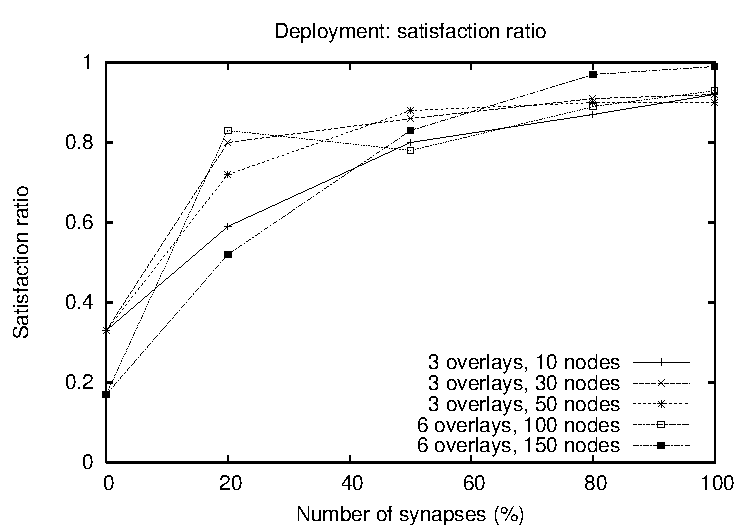
\includegraphics[width=0.5\linewidth]{fig/dep1-sat.pdf}
  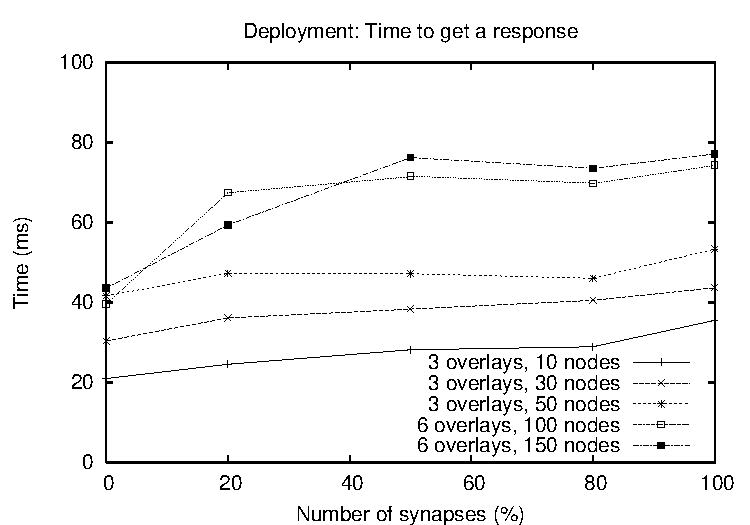
\includegraphics[width=0.5\linewidth]{fig/dep1-time.pdf}
  \up{4}
  \caption{Deploying Synapse : Exhaustiveness and Latency \label{dep:1-sat}}
  \up{4}
\end{figure}

\subsection{Results interpretation}
%
To understand such results, let's consider the following proof: We
call $R$ a region where different peer populations, $P$ and $Q$,
coexist.  At a first stage the two populations have no interactions,
\ie\ $P \cap Q = \emptyset$.  We call $\{ Pub_{P} \}$ and $\{ Sub_{P}
\}$ the number of publications (available trips) and searches
(passengers) in the community/overlay $P$, whereas $\{ Pub_{Q} \}$ and
$\{ Sub_{Q} \}$ are the publications and subscriptions for the
community $Q$.  In a non-interconnected environment, being $\{
Match_{P} \}$ and $\{ Match_{Q} \}$ the number of matches between a
driver and a passenger, an indication of the success of this solution
might be given by $SuccessRate = \# \{ Match_{P} \cup Match_{Q} \}$,
that is the number of matches within the single networks.  By
introducing Synapses to interconnect several communities we change the
assumptions to $P \cap Q \neq \emptyset$ and introduce a new
population $S \subset P \cap Q$, who represents peers residing in $R$
being connected to both $P$ and $Q$ overlays and a new match
figure, $$\{ Match_{P\cup Q} \}=\{ Pub_{P}\,match\,Sub_{Q} \}_{\forall
P,Q \notin S } \cup \{ Pub_{Q}\,match\,Sub_{P}\}_{\forall P,Q
\notin S}$$ which represents the number of matches between an offer
from a peer connected to only one community and a request from a peer
from another community, thanks to the new interconnection provided by
the synapses.  Our success rate becomes then
$$SuccessRate = \# \{ Match_{P} \cup Match_{Q} \cup Match_{P\cup Q} \}$$

The above results show the rate to which $Match_{P\cup Q}$ increases
depending on the number of synapses in an overlay.  Moreover here we
see that with a sufficient rate of co-located nodes the exhaustiveness
of multiple connected communities becomes comparable as if the peers
where all in the same overlay, with the main advantage of scalability
and data locality.  Imagining a worldwide service in fact, it is a big
advantage to handle only local data with the possibility though of
being able to query potentially every other overlay (\ie\ for
occasional long trips).
 
